\section{Background and Related Works}
\label{sec:background}
%UPPRESSO is designed to be compatible with OpenID Connect (OIDC) and provide privacy protections based on the discrete logarithm problem. Next,

This section introduces the popular OIDC \cite{OpenIDConnect},
 to explain typical SSO login flows.
Then, we discuss existing privacy-preserving SSO solutions and other related works.

\subsection{OpenID Connect}
\label{subsec:OIDC}
OIDC is one of the most popular SSO protocols \cite{OpenIDConnect}. %As other SSO protocols \cite{SAMLIdentifier}, OIDC
%It involves three entities, i.e., {\em users}, the {\em identity provider (IdP)}, and {\em relying parties (RPs)}.
Users and RPs register at the IdP with their identities %($ID_U$, $ID_{RP}$ and $PID_U$ in some schemes) %(or $PID_{RP}$ in some schemes)
and other necessary information such as user credentials (i.e., passwords or public keys)
 and RP endpoints (i.e., the URLs to receive identity tokens).
% below can be removed
%The IdP should maintain these attributes securely.

\vspace{1mm}
\noindent\textbf{Implicit Login Flow.}
OIDC supports three types of user login flows: implicit flow, authorization code flow, and hybrid flow (i.e., a mix-up of the previous two).
%In the implicit flow, an {\em id token} is generated as the identity token, which contains a user identifier, an RP identifier, the issuer (i.e., IdP), the validity period, and other requested attributes. The IdP signs the id token using its private key to ensure integrity, and sends it to the RP through the user.
%In the authorization code flow, the IdP binds an authorization code with the RP, and sends it to the RP through the user; then, the RP establishes an HTTPS connection to the IdP and uses the authorization code with the RP's credential to obtain the user's identifier and other attributes.
%UPPRESSO is compatible with all three flows.
These flows mainly result from the differences of the communication steps to request and receive identity tokens,
    but work with the common security requirement of identity tokens.
We introduce the implicit flow and present our design and implementation based on this flow,
    the extensions to support the authorization code flow will be discussed in Section \ref{sec:discussion}.

As shown in Figure \ref{fig:OpenID}, a user firstly initiates a login request to an RP.
Then, the RP constructs an identity-token request with its own identity,
 the endpoint to receive the identity token and the scope of requested user attributes.
This identity-token request is redirected to the IdP.
After successfully authenticating the user,
    the IdP issues an identity token 
        which is forwarded by the user to the RP endpoint.
The token contains a user identity (or pseudo-identity),
    the RP identity, a validity period, the requested user attributes, etc.
%% If the RP endpoint has not been registered at the IdP, the IdP will return a warning to notify the user about potential identity token leakage. % ����ֻ��̸���ߣ����ִ������̫�࣬�ٲ�ʤ��
Finally, the RP verifies the received identity token and
 allows the user to login as the identity in the token.

+++++++++++++++++
Before issuing the identity token,
    the IdP obtains the user's consent to disclose the requested user attributes.
The identity token

Besides redirecting the messages between the RP and the IdP, the user also checks if the RP is permitted to obtain the user attributes in the identity token. Usually, the redirection and checking actions are handled by a user-controlled software called {\em user agent} (e.g., browser).
%extracts user's identifier and returns the authentication result to the user (Step 7).


If a privacy-preserving pseudo-identity is used, this process also involves mapping the real identifier ($ID_U$) to the pseudo identifier ($PID_U$).
%$ID_U$ to $PID_U$ based on $ID_{RP}$.

\vspace{1mm}
\noindent\textbf{RP Dynamic Registration.}
OIDC also supports {\em RP dynamic registration} \cite{DynamicRegistration}. When an RP first registers at an IdP, it obtains a registration token with which the RP can %initiate a dynamic registration process to
update its information (e.g., endpoints) with the IdP at a later time. After a successful dynamic registration, the RP obtains a new $ID_{RP}$ from the IdP.
+++++
We only talk about the background. nothing on UPPRESSO.
+++++
UPPRESSO leverages this function and slightly modifies the dynamic registration process to implement the {\em $PID_{RP}$ registration} process (see details in Section \ref{sec:UPPRESSO}.C), which allows an RP to generate different privacy-preserving RP identifiers and register them with the IdP.

\begin{figure}[t]
  \centering
  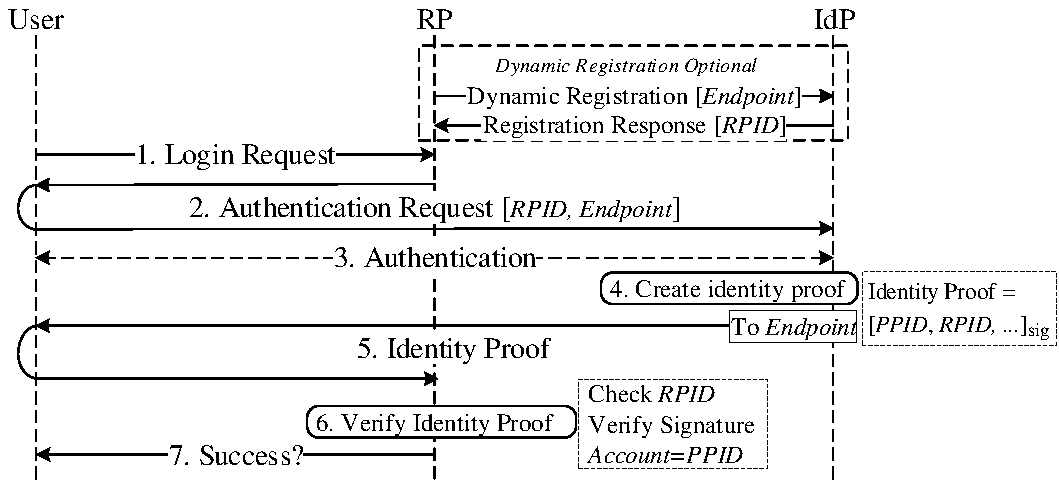
\includegraphics[width=0.9\linewidth]{fig/OIDC1.pdf}
  \caption{The implicit flow of OIDC.}
  \label{fig:OpenID}
  \vspace{-5mm}
\end{figure}

\subsection{Existing Privacy Solutions for SSO}
\label{subsec-solutions}
Pairwise pseudonymous identifier (PPID) is recommended by NIST \cite{NIST2017draft} and specified in several SSO protocols \cite{OpenIDConnect, SAMLIdentifier} to hide the real user identity from the RPs. It can be generated by the IdP to identify a user to an RP. PPIDs for one user at different RPs should not be correlated with each other, so that collusive RPs cannot link a user's logins. However, PPID-based approaches cannot prevent IdP-based login tracing, since the IdP needs to know which RP the user visits to generate the correct identify token.

Meanwhile, BrowserID \cite{BrowserID} and SPRESSO \cite{SPRESSO} proposed to defend against IdP-based login tracing. However, both solutions are vulnerable to RP-based identity linkage. In BrowserID (and its prototypes known as Mozilla Persona \cite{persona} and Firefox Accounts \cite{FirefoxAccount}), the IdP does not know the identity of the requesting RP. Instead, it generates a special ``identity token'' to bind the user's unique identifier (e.g., email address) to a public key, so that the user can sign another subsidiary identity token to bind her identity with the RP's identity and send both identity tokens to the RP. Obviously, when a user logs in to different RPs, the RPs can extract the same user identifier from different identity tokens and correlate these logins. In SPRESSO, the RP creates a one-time pseudo-identity for itself at each login. Then, the IdP generates an identity token binding this pseudo-identity of the RP and the user's identity (i.e., email address). %and returns it through a trusted third-party entity called forwarder.
Similarly, the RPs can correlate a user's logins using her unique identifier in the identity tokens.

\begin{comment}

\subsection{Discrete Logarithm Problem}
\label{sec:dlp}


Based on the discrete logarithm problem, UPPRESSO designs the identifier-transformation functions. %$\mathcal{F}_{ID_{RP} \mapsto PID_{RP}}$ and $\mathcal{F}_{ID_{U} \mapsto PID_{U}}$ to generate privacy-preserving user identifier (e.g. $PID_U$) and RP identifier (e.g. $PID_{RP}$), respectively.
Here, we briefly review the discrete logarithm problem.
%A number $g$ ($0<g<p$) is called a primitive root modular a prime $p$, if for ${\forall}y$ ($0<y<p$), there is a  number $x$ ($0\le x <p-1$) satisfying $y=g^x \pmod p$.
For the finite field $GF(p)$ where $p$ is a large prime, a number $g$ is called a generator of order $q$, if it constructs a cyclic  group of $q$ elements by calculating $y=g^x \ mod\ p$.
And $x$ is called the discrete logarithm of $y$ modulo $p$. Given a large prime $p$, a generator $g$ and a number $y$, it is computationally infeasible to solve the discrete logarithm (i.e., $x$) of $y$ \cite{WXWM}, which is called the discrete logarithm problem.
The hardness of solving discrete logarithms is utilized to design several secure cryptographic primitives, including Diffie-Hellman key exchange and the digital signature algorithm (DSA).

%In the process of $F_{PID_{RP}}$ and $F_{PID_U}$, we needs to calculate the primitive root for a  large prime $p$ as follows \cite{Shoup,Wang}. First, we retrieve a primitive root $g_m$  modulo $p$ from all the integers by finding the first integer passing  the primitive root checking.  A lemma is propose to simply the checking, that if $p=2q+1$ ($q$ is a prime),  an integer $\mu \in (1, p-1)$ is a primitive root if and only if $\mu^2\neq 1 \ mod \ p$ and $\mu^q\neq 1 \ mod \ p$. Then, based on $g_m$, we can calculate a new primitive root $g = g_{m}^{t} mod \ p$, where $t$ is an integer coprime to $p-1$.
\end{comment}
